% Observer/Estimator
% Author: Dominik Haumann
\documentclass[landscape,a5paper,11pt]{article}
\usepackage[utf8x]{inputenc} % utf8 encoding
\usepackage[T1]{fontenc} % use T1 fonts
\usepackage{amsmath} % nice math symbols
\usepackage{bm} % bold math
\usepackage{color} % change text color        

\usepackage{tikz}


\tikzset{
	block/.style  = {draw, fill=white, rectangle, minimum height=3em, minimum width=5em, node distance = 2cm},
	sum/.style    = {draw, fill=white, circle, node distance=1cm},
	input/.style  = {coordinate},
	output/.style = {coordinate},
	hidden/.style  = {coordinate},
}

\begin{document}
	
	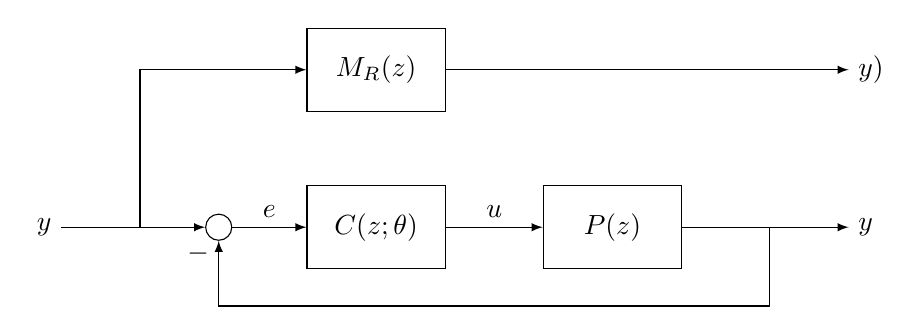
\begin{tikzpicture}[auto, >=latex]
		% Draw the main control loop nodes
		\draw
			node[input] (input) {}
			node[hidden, right of = input     ] (inputfork) {}
			node[sum   , right of = inputfork ] (sum) {}
			node[block , right of = sum       ] (controller) {$C(z; \theta)$}
			node[block , right of = controller, node distance = 3cm] (plant) {$P(z)$}
			node[hidden, right of = plant     , node distance = 2cm] (outputfork) {}
			node[output, right of = outputfork] (output) {}
			node[hidden, below of = plant     ] (retroaction) {};
		
		% Draw the reference model nodes
		\draw
			node[block , above of = controller] (refmodel) {$M_R(z)$}
			node[coordinate, right of = refmodel, node distance = 6cm] (refoutput) {};
			
		% Connect everything together
		\draw[->] node[left] {$y°$} (input) -- (inputfork)  -- (sum);
		\draw[->] (sum) -- (controller) node[midway] {$e$};
		\draw[->] (controller) -- (plant) node[midway] {$u$};
		\draw[->] (plant) -- (outputfork) -- (output) node[right] {$y$};

		\draw[->] (outputfork) |- (retroaction) -| node[pos=0.9] {$-$} (sum);
		
		\draw[->] (inputfork) |- (refmodel);
		\draw[->]  (refmodel) -- (refoutput) node[right] {$y$)};
	\end{tikzpicture}
	
	\begin{tikzpicture}[scale=1, auto]
		\node[draw, circle] (Sum) at (-2, 0) {};
		\node[draw] (Controller)  at  (0, 0) {$C(z; \theta)$}; 
		\node[draw] (Plant)       at  (3, 0) {$P(z)$};
		\node[draw] (RefModel)    at  (2, 2) {$M_R(z)$};
				
		\coordinate[shift={(0,-1)}] (n) at (Plant.south);
		
		\draw[->, >=stealth] (-4, 0)      -- (Sum); 
		\draw[->, >=stealth] (Sum)        -- (Controller) node[midway] {$e(t)$}; 
		\draw[->, >=stealth] (Controller) -- (Plant) node[midway] {$u(t)$}; 
		\draw[->, >=stealth] (Plant)      -- (6, 0);
		\draw[->, >=stealth] (4, 0)       |- (n) -| (Sum);
		
		\draw[->, >=stealth] (-3, 0) |- (RefModel);
		\draw[->, >=stealth] (RefModel) -- (6, 2) node[right] {$y(t)$};
		
		
		\draw (-4, 0) node[left] {$r_i(t)$};
		\draw (6, 0)  node[right] {$y(t)$};
		\draw (Sum) node[below left] {$-$};
		\draw (Sum) node[above left] {$+$};
	\end{tikzpicture}

\end{document}